\documentclass[12pt,a4paper]{article}
\usepackage[italian]{babel}
\usepackage[utf8]{inputenc}
\usepackage{fourier} 

% Images
\usepackage{graphicx}
\usepackage{caption}
\usepackage{subcaption}
\usepackage{float}
\graphicspath{ {../Images} }

% FlowChart
\usepackage{smartdiagram}

% Stop hyphenation
\usepackage[none]{hyphenat}

\begin{document}

\title{\textbf{\centering{Manuale per operatori.}\\Tour guidato per bambini ai Musei civici.}}
\author{Alice Balestieri}
\date{}

\maketitle
\newpage

\tableofcontents
\newpage

\section{Schema posizionamento Opere all'interno del Museo.}

\begin{center}
	\smartdiagramset{set color list={green!60!lime,red!80!black, blue!50!cyan, brown!80, violet!80}, back arrow disabled=true, module minimum width=10cm, module minimum height=1.5cm, module y sep=2.30, arrow line width=0.16cm, text width=8cm}
	\smartdiagram[flow diagram]{Scalone ingresso opera ceramica:\\ \textbf{La Medusa di Ferruccio Mengaroni}, Sala Giovanni Bellini: \\ \textbf{Opere di natura Ecclesiastica e provenienti dalla collezione Rossini},
		 Sala delle ceramiche collezione di Domenico Mazza: \\ \textbf{Piatto in ceramica con scoiattolo nero}, Sala arredi e sculture collezione Mosca, Sala natura e inganno}
\end{center}

\section{Che cosa spiegare:}

	\begin{enumerate}
		
	\item 	Mostrare la Medusa di Ferruccio Mengaroni, situata accanto allo scalone d'ingresso ai Musei sulla sinistra, raccontando della maledizione legata all'imponente opera ceramica.\par
	\begin{minipage}{\linewidth}
		\centering
		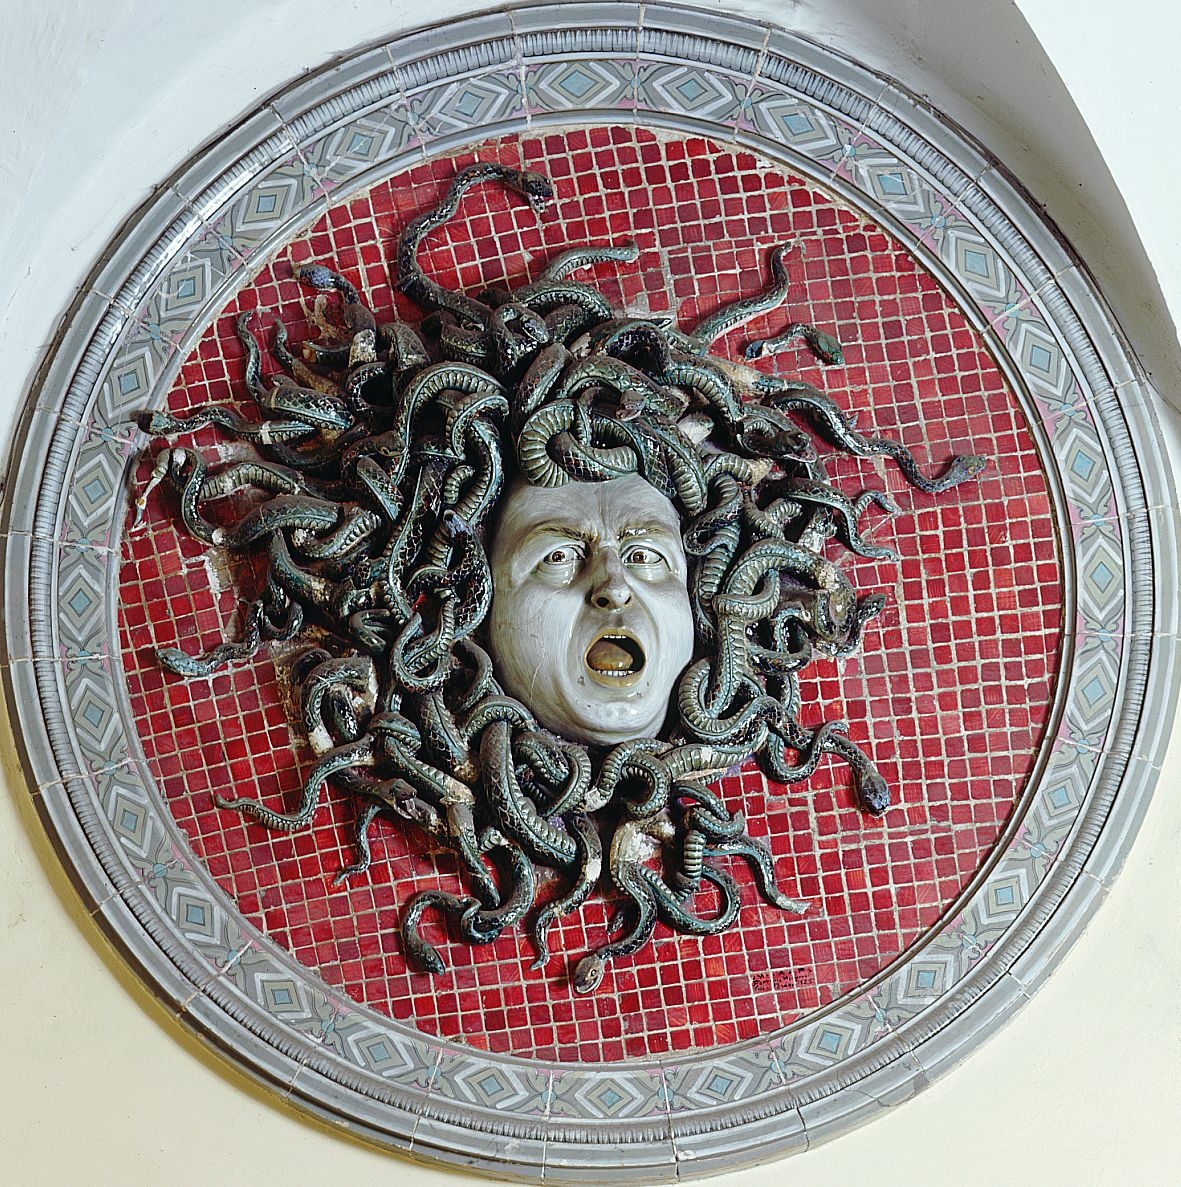
\includegraphics[]{Medusa.jpg}
		\captionof{figure}{Medusa di Ferruccio Mengaroni.}
	\end{minipage}
	
	\item Mostrare la \textbf{Pala Bellini} (presente nella sala Bellini). Evidenziando il dettaglio della \textit{Colomba} che rappresenta lo \textit{Spirito Santo}, presente nel pannello centrale contenente la scena dell'Incoronazione della Vergine e il dettaglio del \textit{Drago di S. Giorgio e il Drago}, presente in basso tra i sette riquadri della predella.\par
	\begin{minipage}{\linewidth}
		\centering
		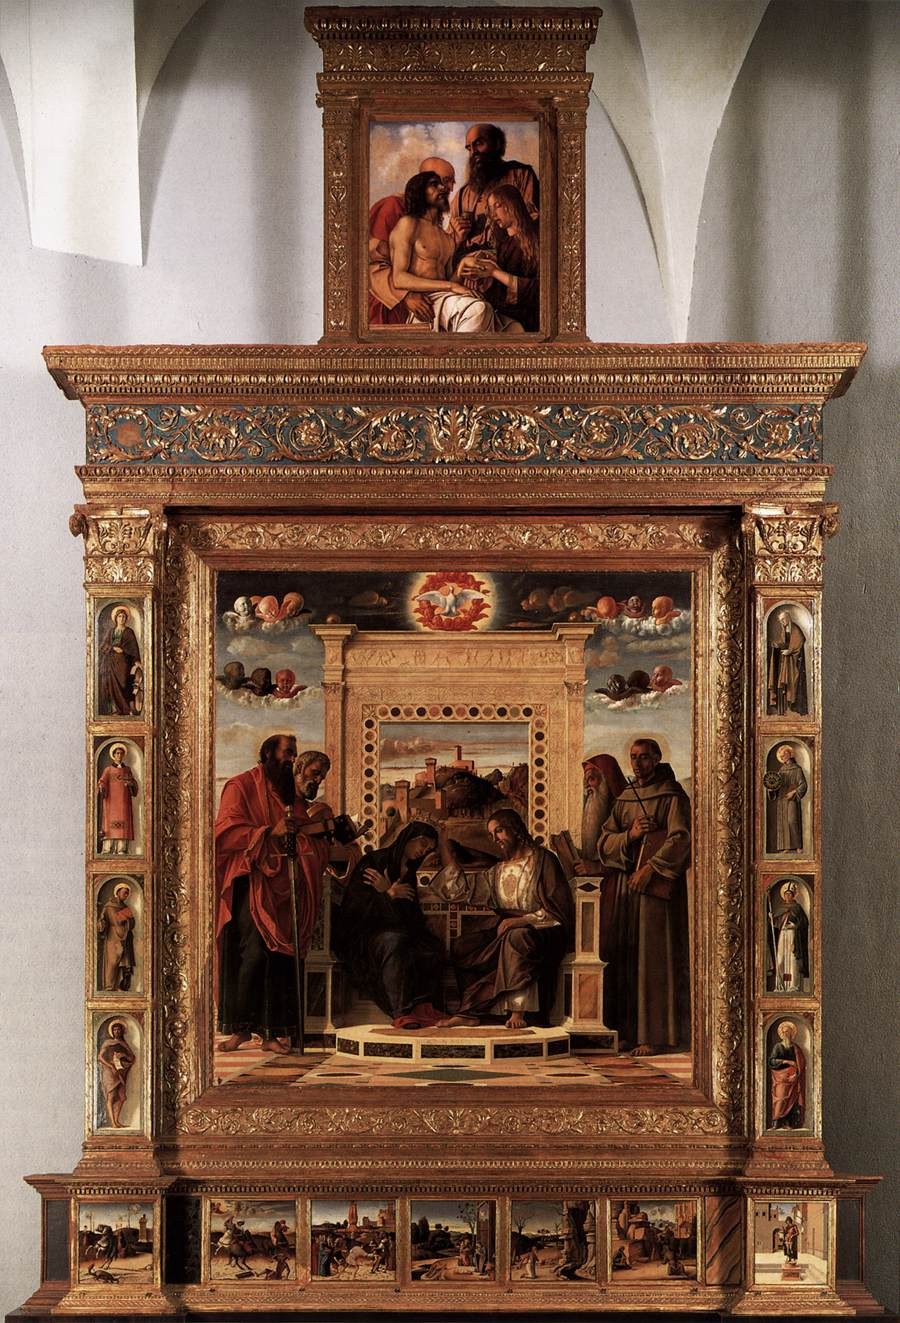
\includegraphics[scale=0.8]{Pala_di_pesaro.jpg}
		\captionof{figure}{Pala di Pesaro.}
	\end{minipage}
	
	\begin{minipage}{\linewidth}
		\centering
		\begin{minipage}{0.4\linewidth}
			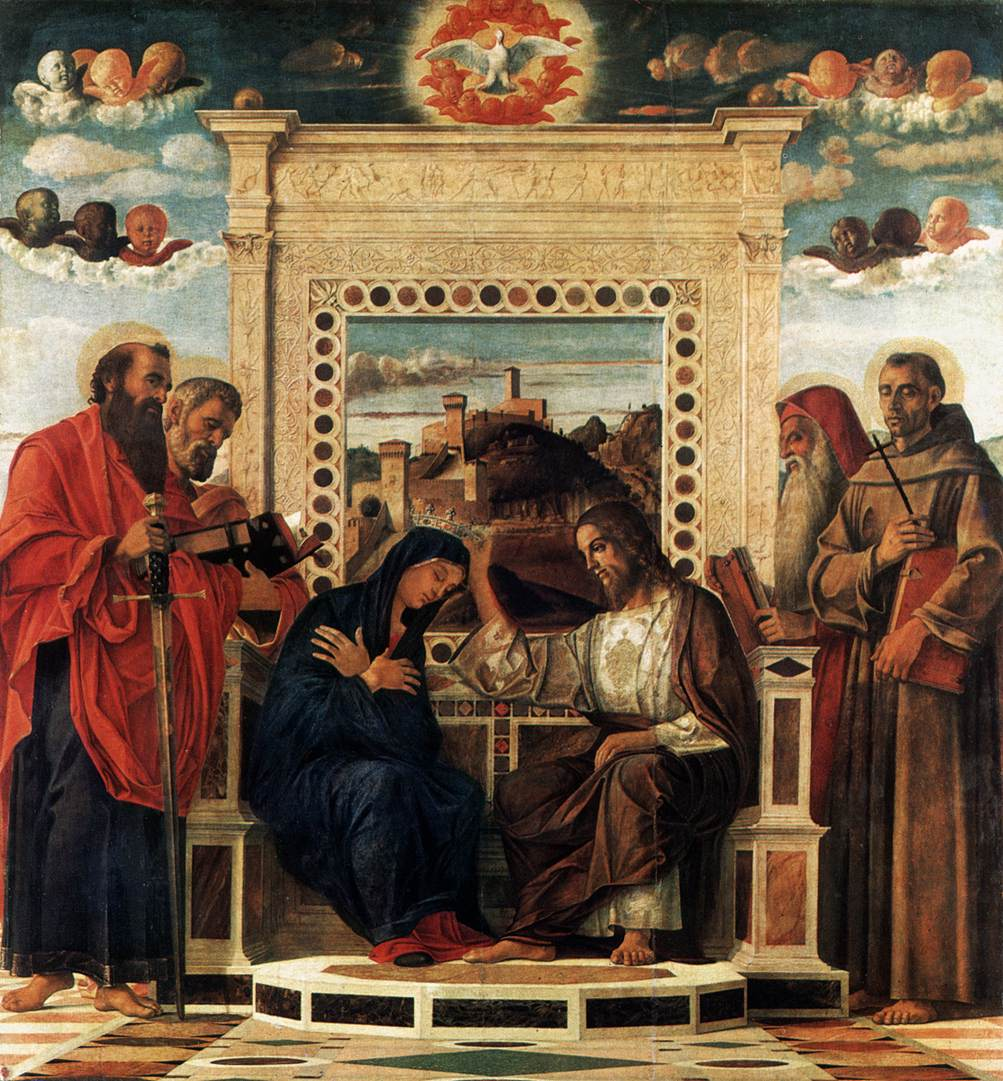
\includegraphics[scale=0.65]{Pala_di_pesaro_incoronazione.jpg}
			\captionof{figure}{Pala di Pesaro - Incoronazione della Vergine.}
		\end{minipage}
		\hfill
		\begin{minipage}{0.4\linewidth}
			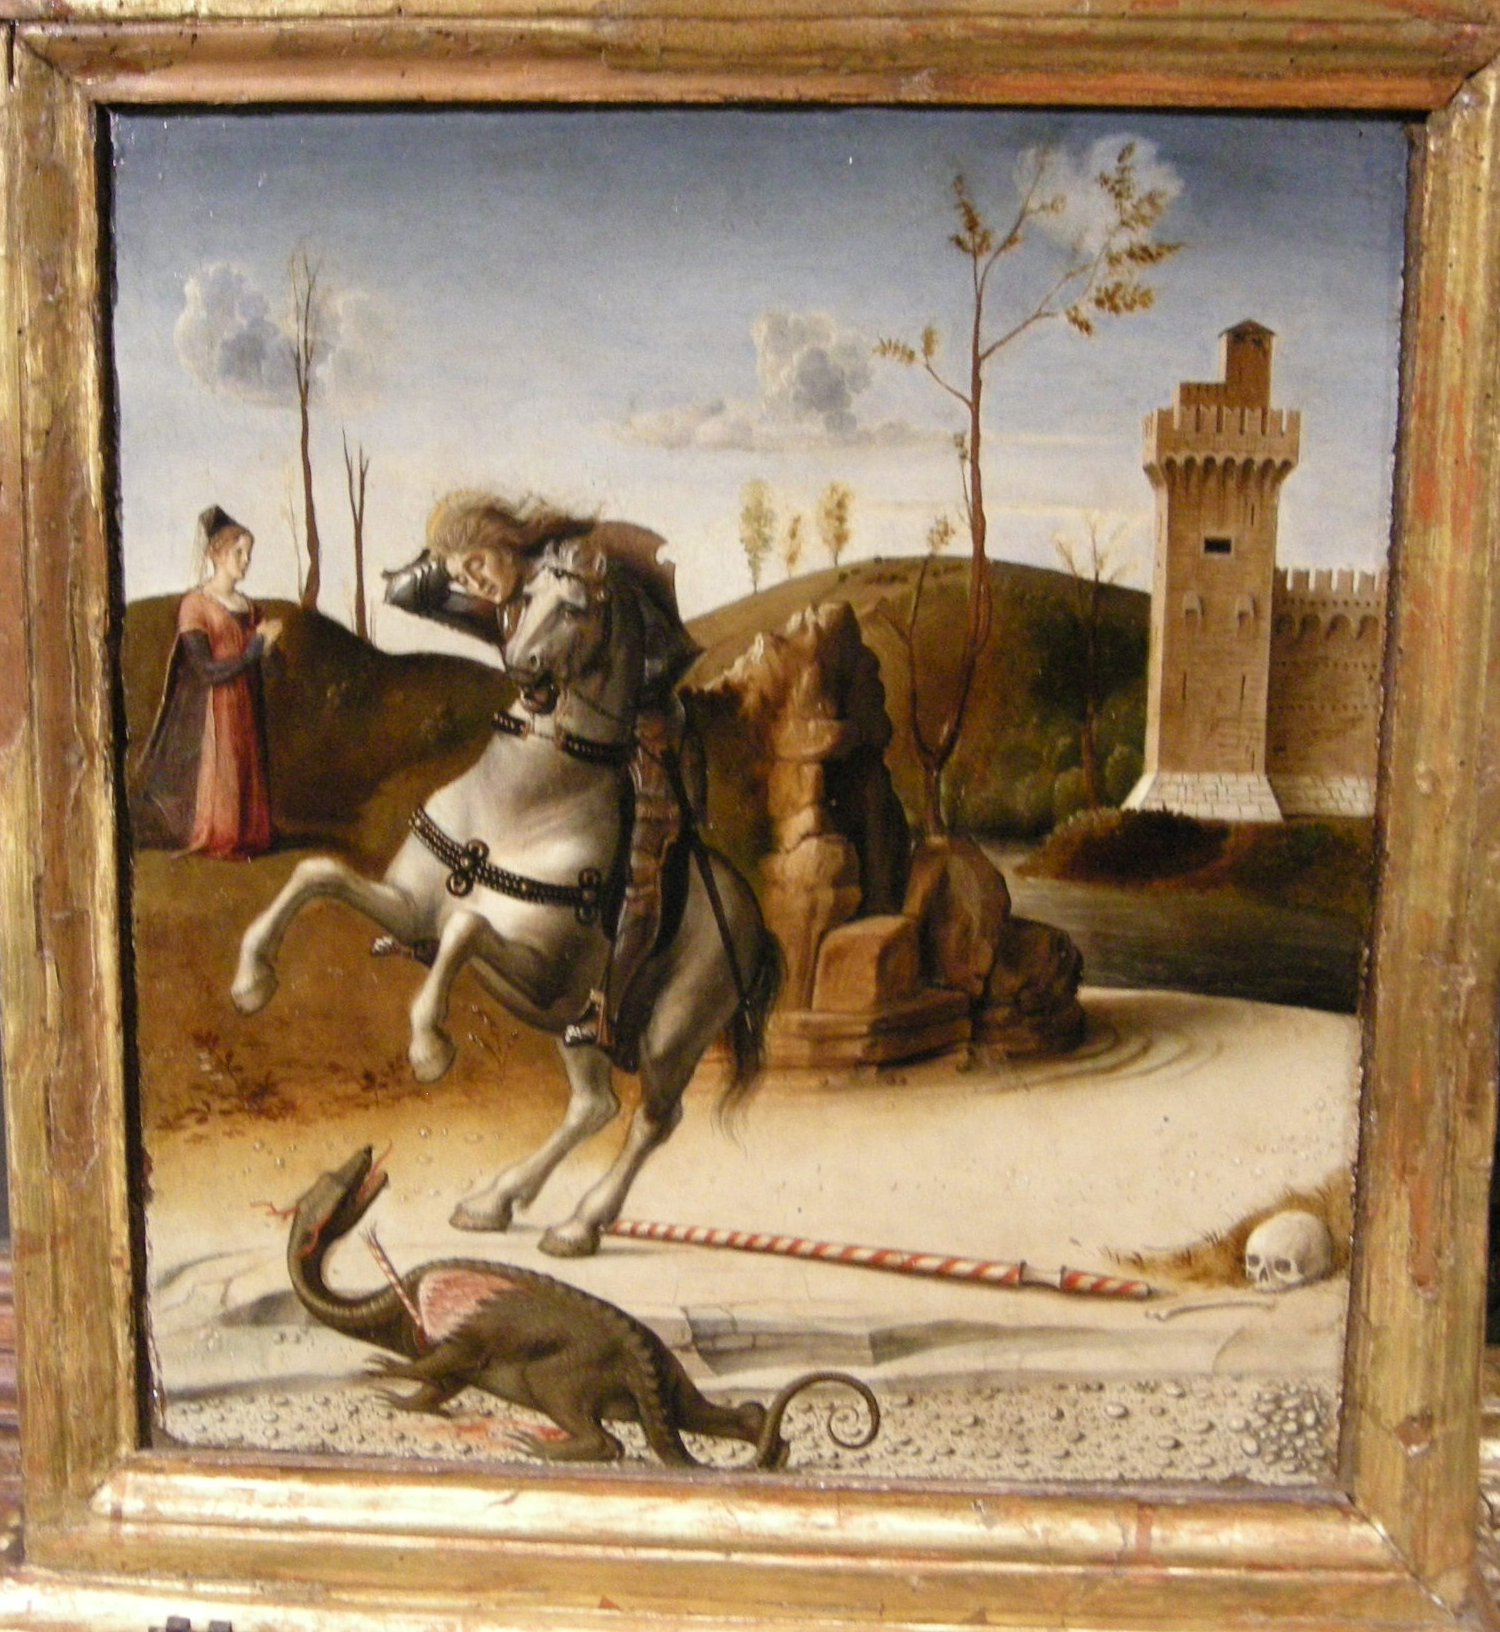
\includegraphics[scale=0.1]{Pala_di_pesaro_predella.jpg}
			\captionof{figure}{Pala di Pesaro - S. Giorgio e il Drago.}
		\end{minipage}
	\end{minipage}
	
	\item Mostrare quadri che fanno uso della prospettiva, confrontandoli con quelli che ne sono privi. \par
	\begin{minipage}{\linewidth}
		\centering
		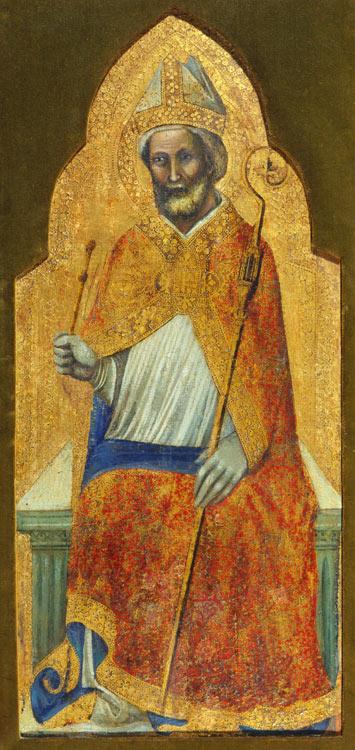
\includegraphics[scale=0.35]{SanAmbrogio.jpg}
		\captionof{figure}{Sant'Ambrogio, arcivescovo di Milano. \\ \centering Esempio di quadro senza prospettiva.}
	\end{minipage} 
	
	
	\item Spiegare gli elementi che contraddistinguono la \textbf{Collezione Rossini}; come il \textit{Rosso vermiglio} e \textit{l'oro ed i gioielli} nei dipinti.\par
	\begin{minipage}{\linewidth}
		\centering
		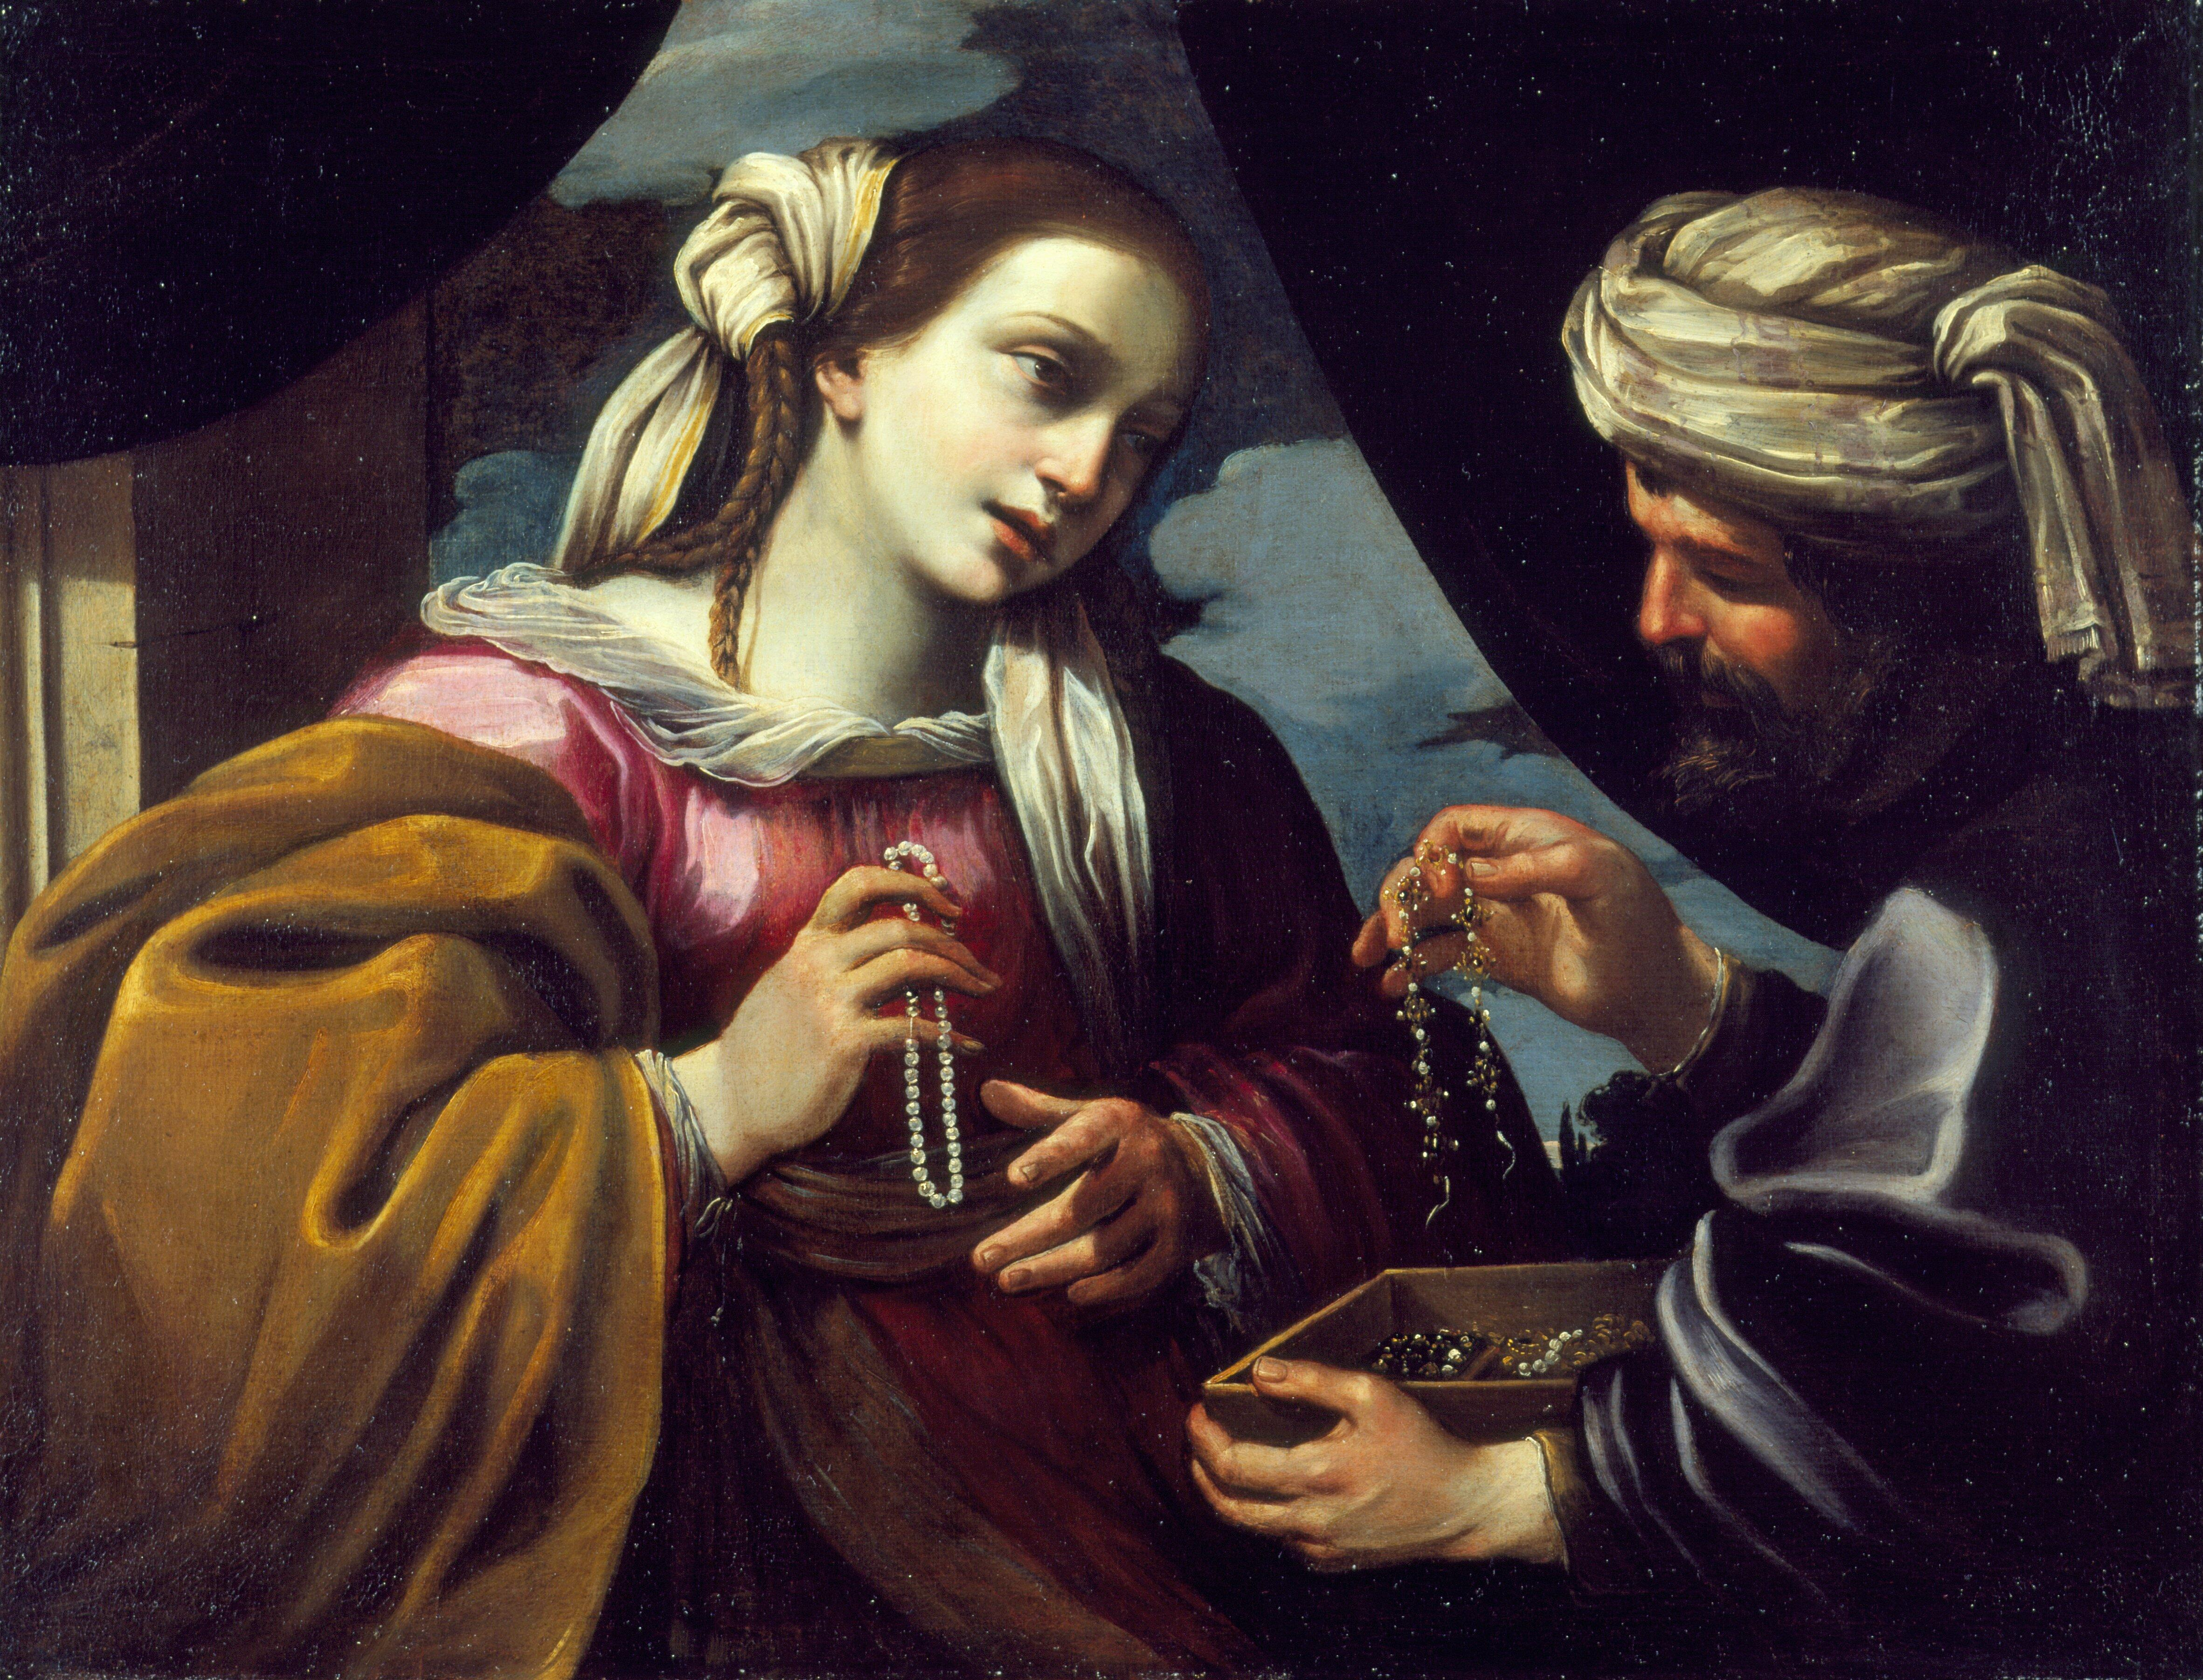
\includegraphics[scale = 0.05]{Pietro_Desani_Rebeca_y_Eleazar.jpg}
		\captionof{figure}{Pietro Desani - Rebeca y Eleazar.}
	\end{minipage}
	
	\item Mostrare la \textbf{ceramica della collezione Mazza} dove è presente lo \textit{scoiattolo nero di cinquecento anni fa}.\par
	\begin{minipage}{\linewidth}
		\centering
		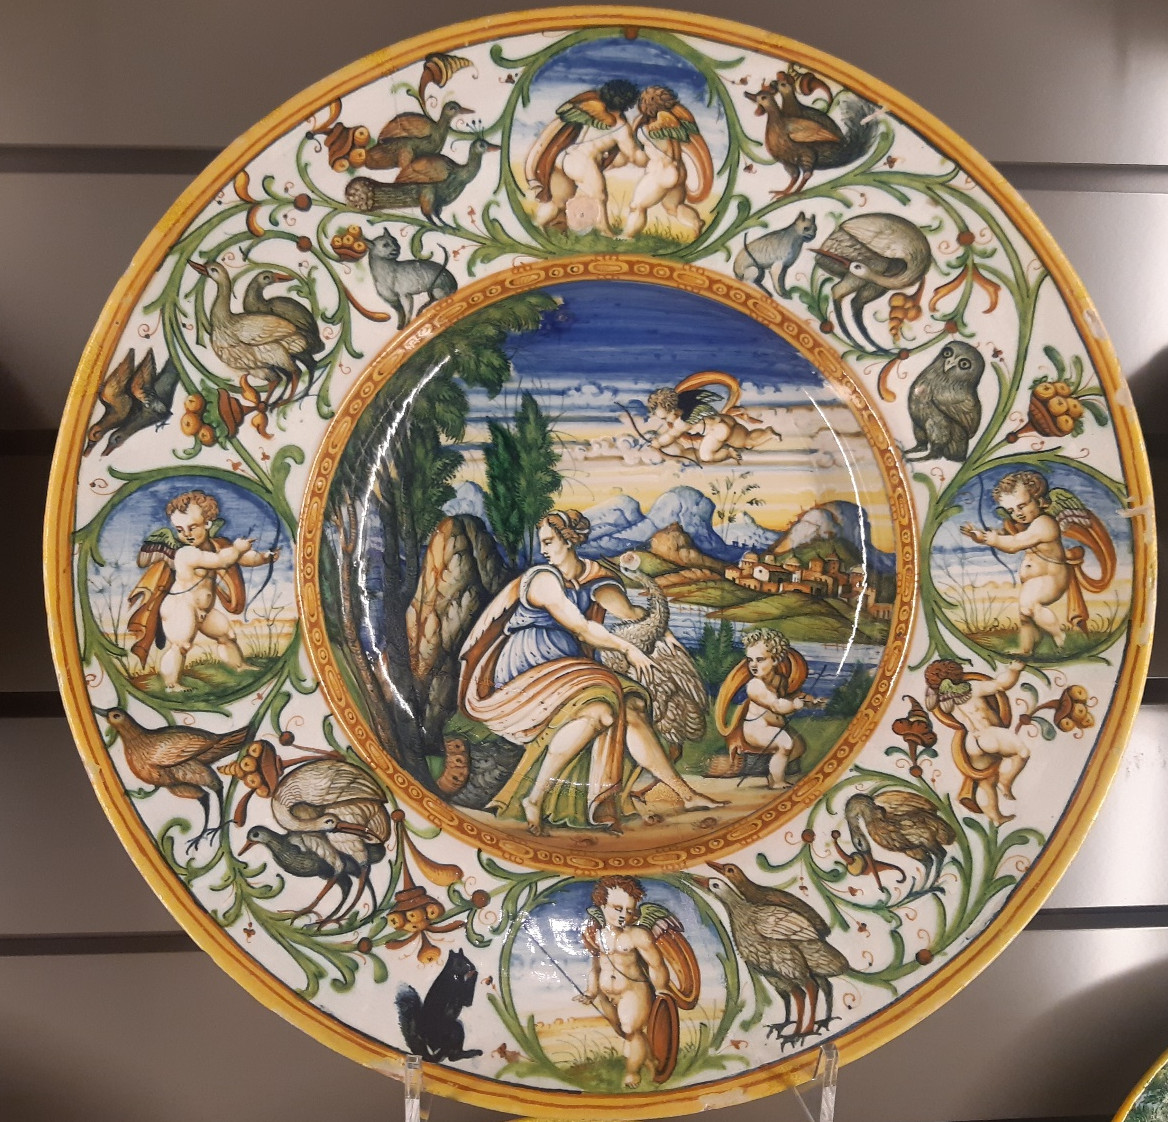
\includegraphics[scale=0.6]{Piatto_Scoiattolo_Nero.jpg}
		\captionof{figure}{Piatto collezione Mazza dove è presente uno scoiattolo nero.}
	\end{minipage}
	
	\item Esporre in maniera semplice: lo \textbf{specchio in vetro di Murano} decorato con \textit{incisioni d'uva d'argento},  gli \textbf{oggetti in avorio e madreperla}, lo \textbf{Stipo con vedute di Roma} facendo riferimento alle \textit{cartoline} di Roma e l'\textbf{Orologio Notturno}.\par
	\begin{minipage}{\linewidth}
		\centering
		\begin{minipage}{0.4\linewidth}
			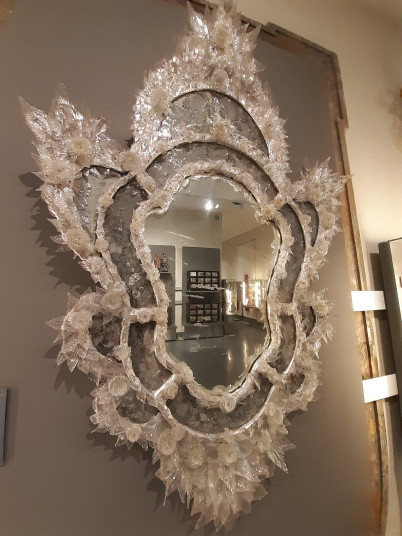
\includegraphics[scale=1.3]{Specchio_Murano.jpg}
			\captionof{figure}{Specchio in vetro di Murano.}
		\end{minipage}
		\hfill
		\begin{minipage}{0.4\linewidth}
			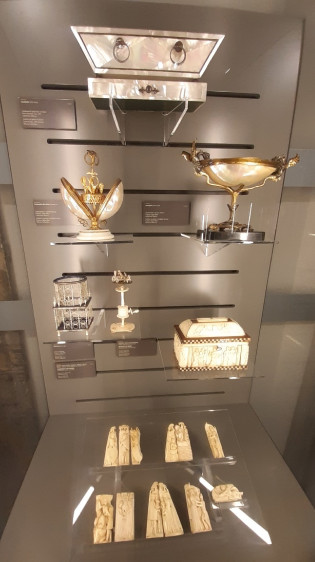
\includegraphics[scale=1.25]{Avorio_madreperla.jpg}
			\captionof{figure}{Oggetti in avorio e madreperla.}
		\end{minipage}
	\end{minipage}
	
	\begin{minipage}{\linewidth}
		\centering
		\begin{minipage}{0.4\linewidth}
			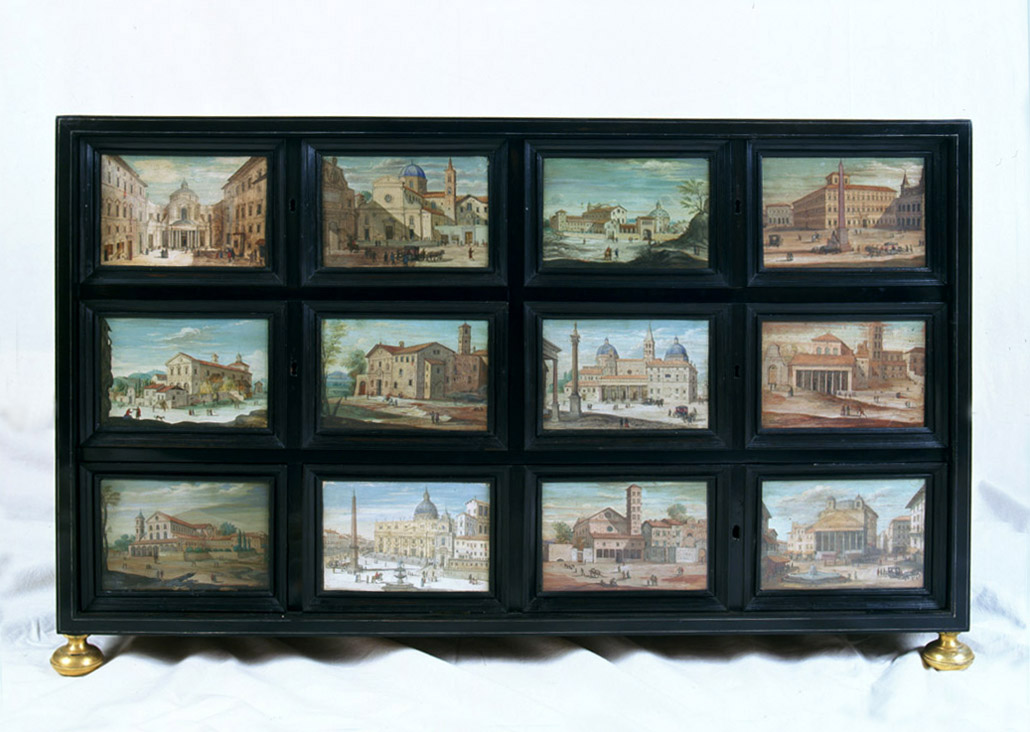
\includegraphics[scale=0.2]{Vedute_di_Roma.jpg}
			\captionof{figure}{Vedute di Roma.}
		\end{minipage}
		\hfill
		\begin{minipage}{0.4\linewidth}
			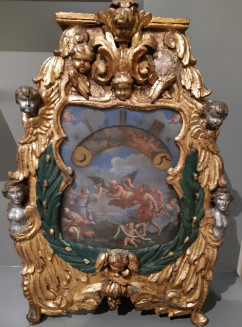
\includegraphics[scale=1.85]{Orologio_Notturno.jpg}
			\captionof{figure}{\raggedright{Orologio notturno.}}
		\end{minipage}
	\end{minipage}
	
	\item Mostrare il \textbf{Piatto della bottega pesarese} con \textit{decoro della Rosa di Pesaro}.\par
	\begin{minipage}{\linewidth}
		\centering
		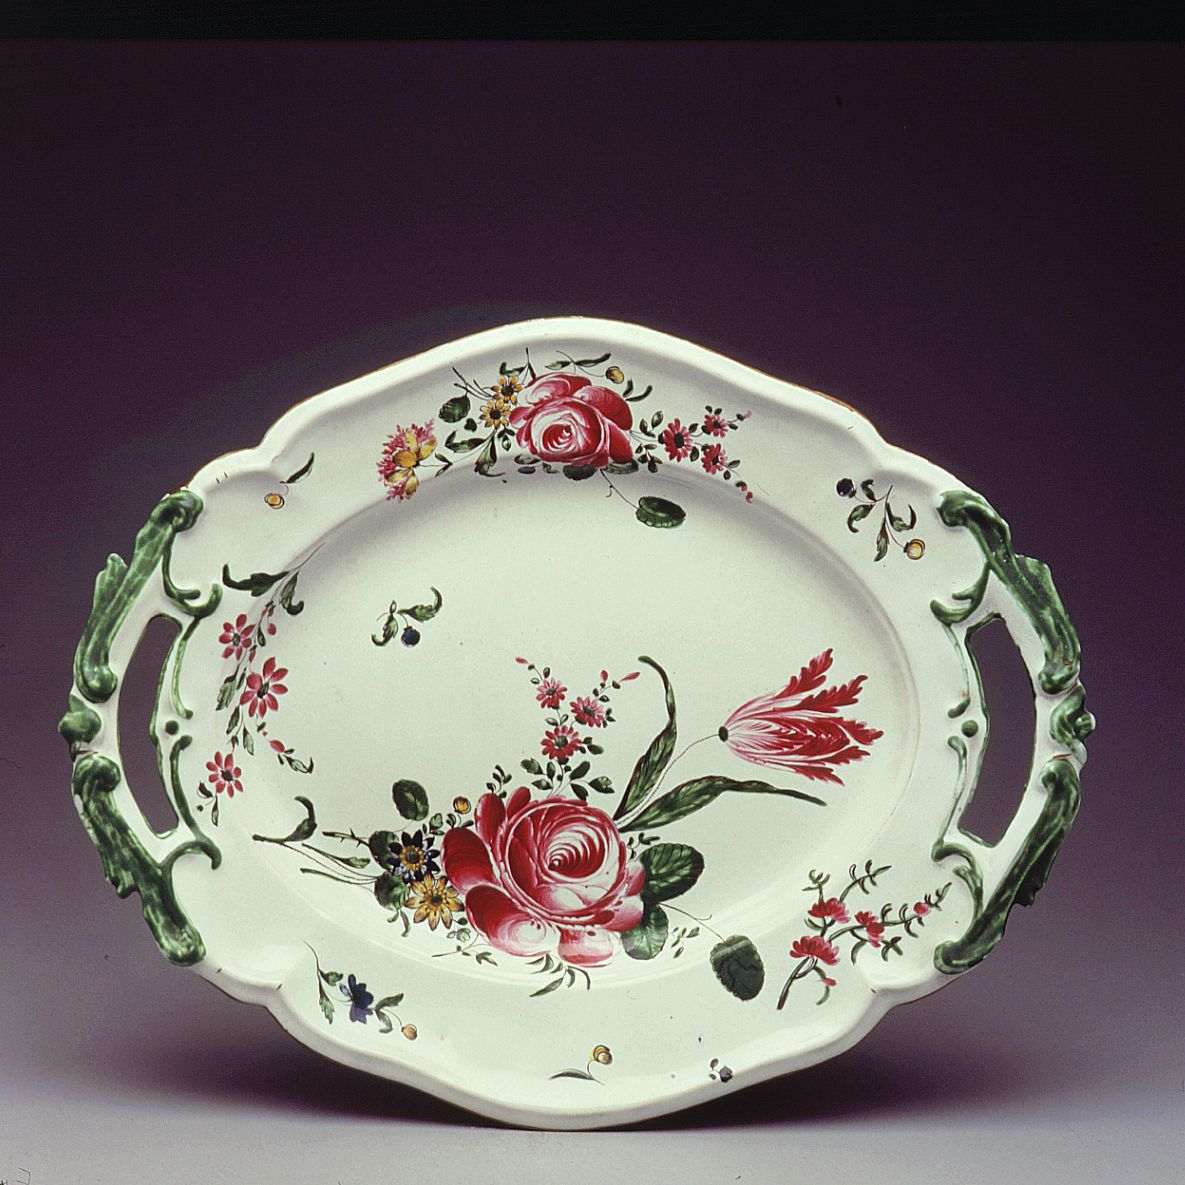
\includegraphics[]{Piatto_pesaro.jpg}
		\captionof{figure}{Piatto - bottega pesarese.}
	\end{minipage}
	
	\item Mostrare il dipinto ad olio Il Mercato di Aureliano Milani, che rappresenta una scena di vita quotidiana all'interno di un piccolo borgo abitato, in cui sono visibili diversi ceti sociali e i loro relativi mestieri.\par
	\begin{minipage}{\linewidth}
		\centering
		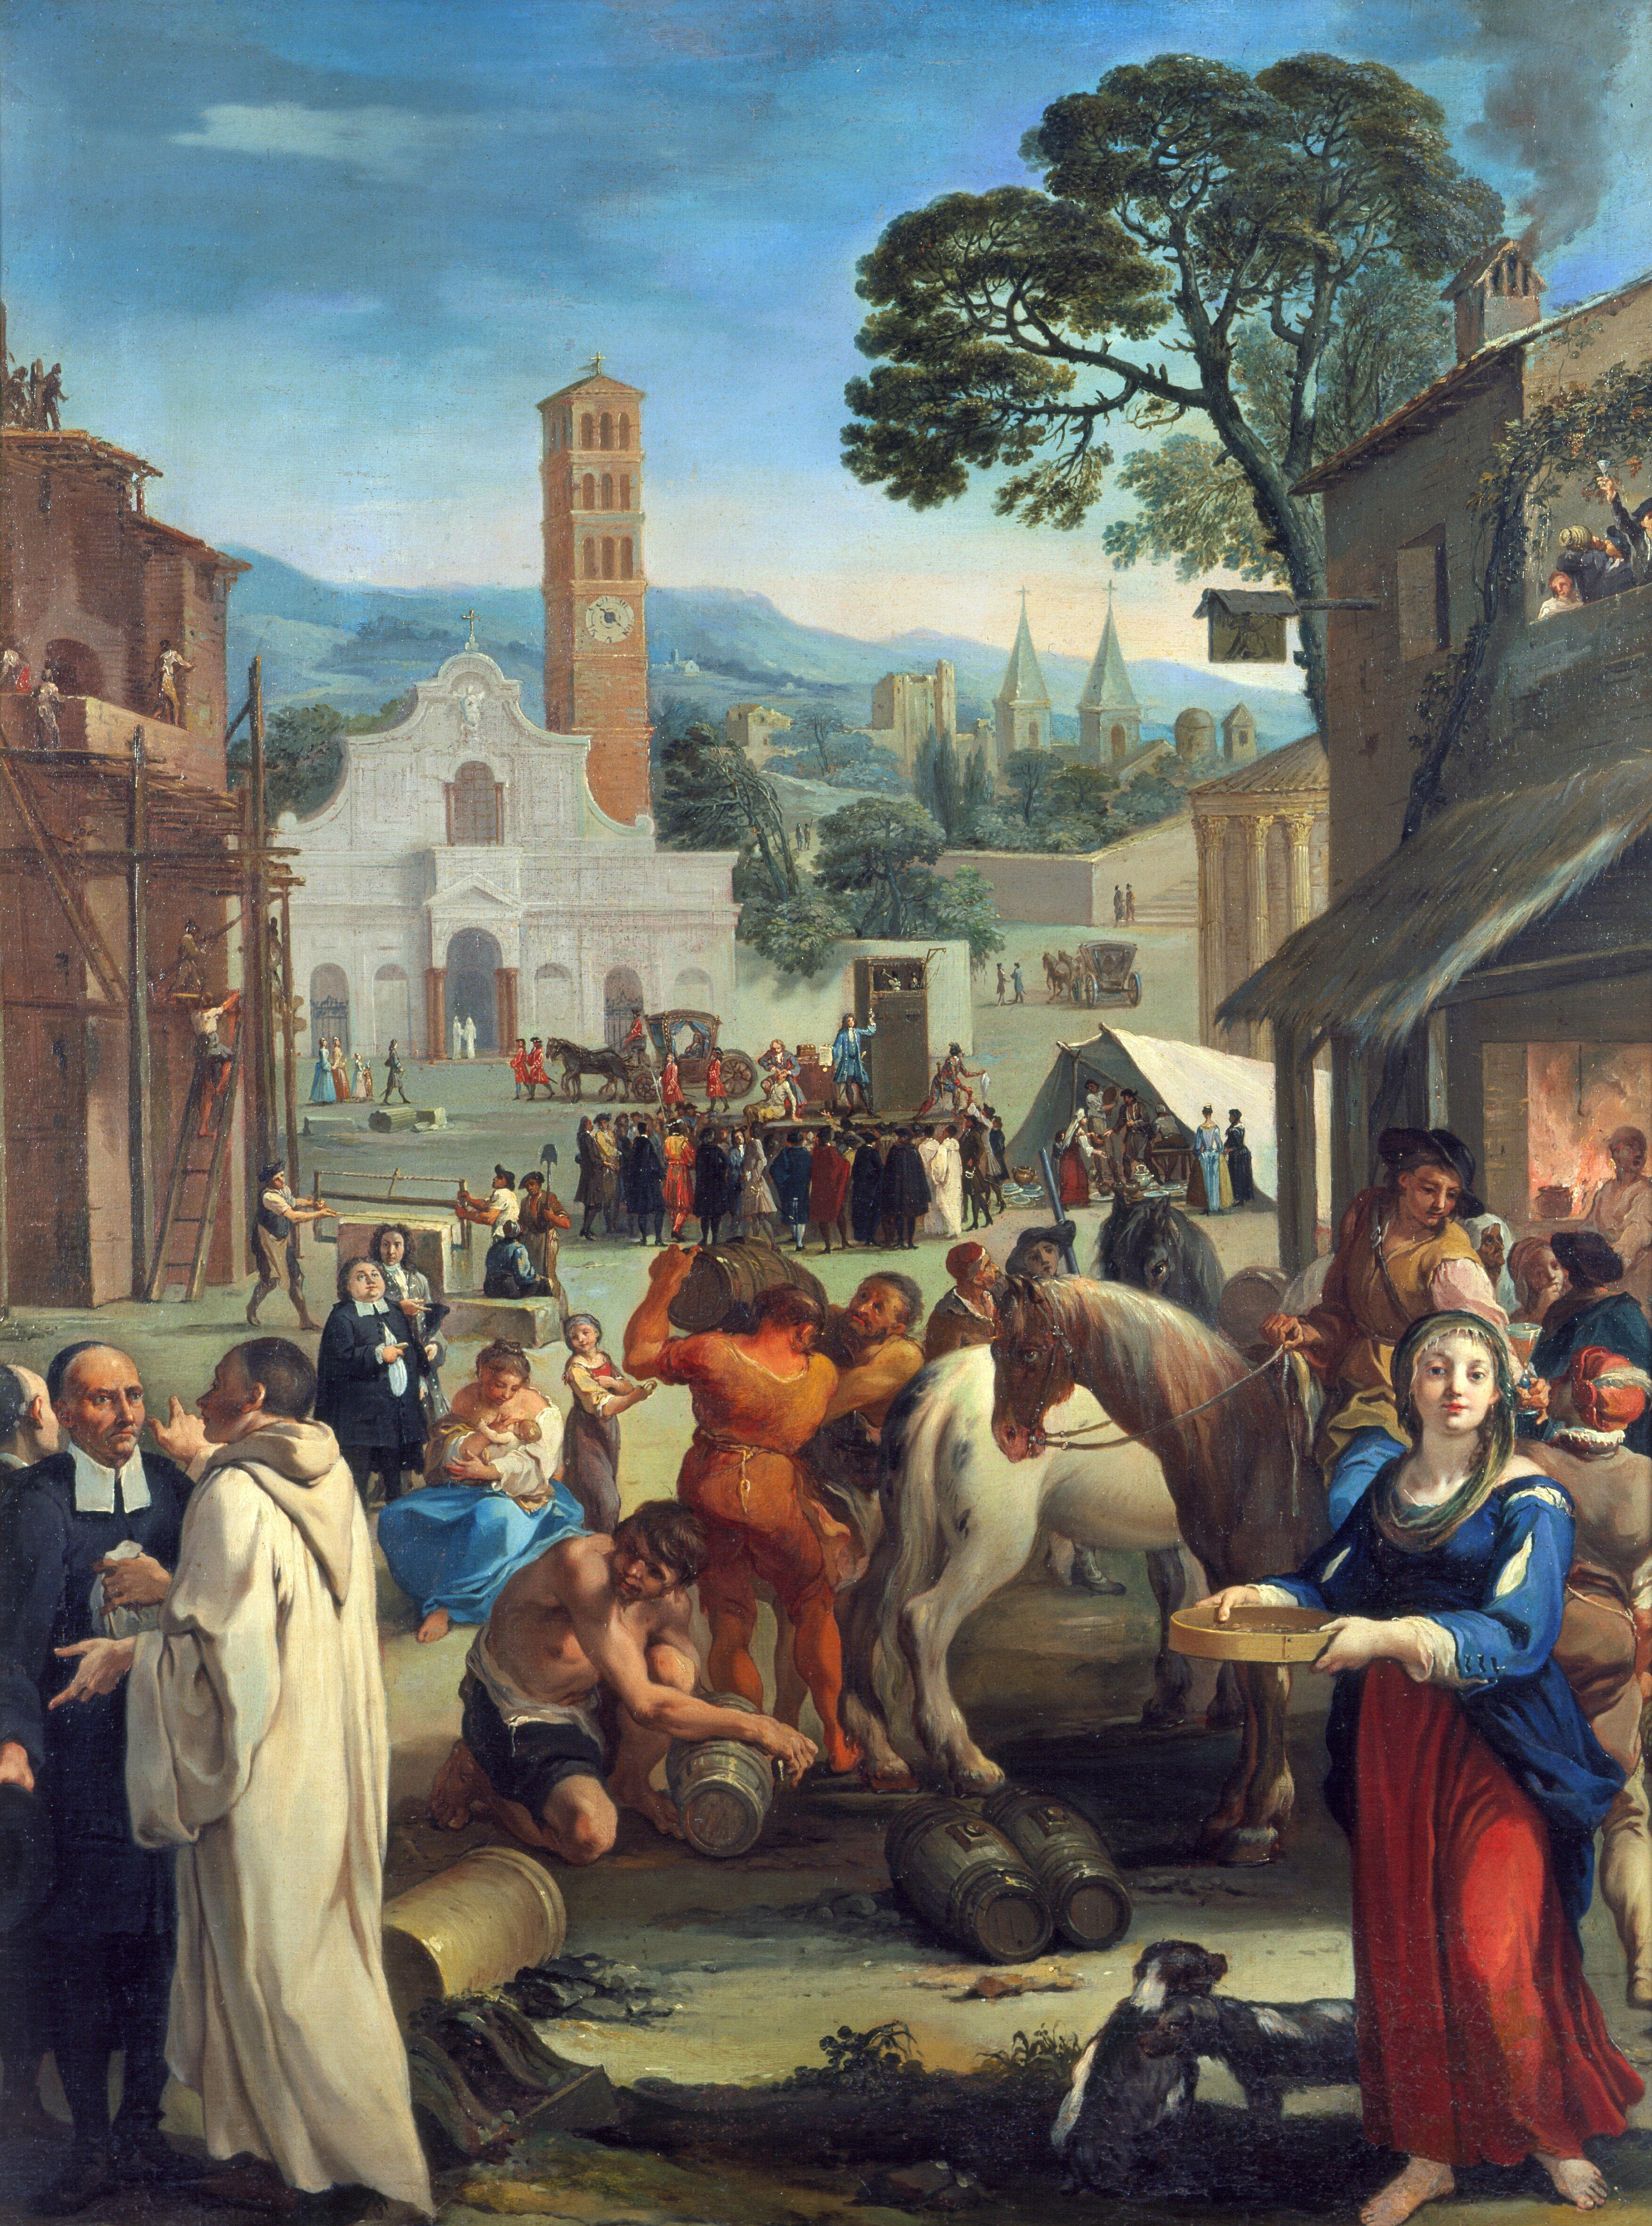
\includegraphics[scale=0.05]{Aureliano_Milani_Mercato.jpg}
		\captionof{figure}{Aureliano Milani - Il mercato.}
	\end{minipage}

	
	\item Mostrare le \textbf{Nature Morte}, evidenziando la \textit{frutta} ed i \textit{calici in vetro}, mostrare il \textbf{Trompe l'oeil} con il \textit{Sonetto di Antonio Gianlisi Junior} e il \textbf{Trompe l'oeil} con la \textit{pipa} mettendo in risalto i cibi e gli oggetti di uso comune come la \textit{pipa} e i \textit{savoiardi} che alludono ai Savoia.\par
	\begin{minipage}{\linewidth}
		\centering
		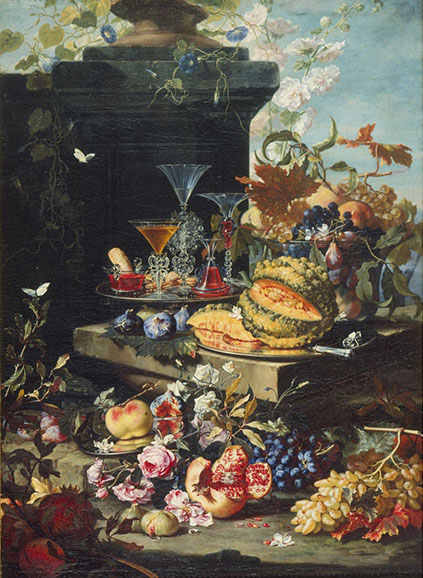
\includegraphics[scale= 0.3]{Fiori_Frutta.jpg}
		\captionof{figure}{Fiori, frutta e un vassoio con calici di vetro.}
	\end{minipage}
	
	\begin{minipage}{\linewidth}
		\centering
		\begin{minipage}{0.4\linewidth}
			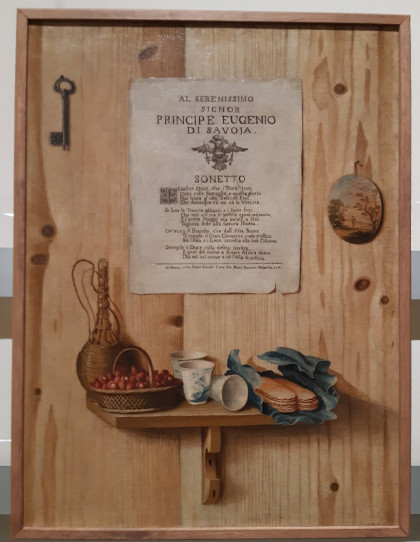
\includegraphics[scale=1.3]{Trompe_savoiardi.jpg}
			\captionof{figure}{Trompe l'oeil con savoiardi.}
		\end{minipage}
		\hfill
		\begin{minipage}{0.4\linewidth}
			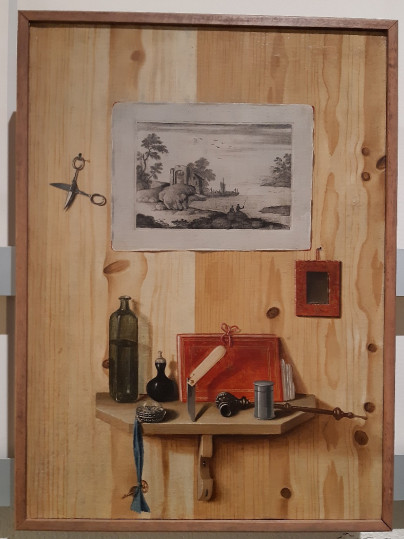
\includegraphics[scale=1.3]{Trompe_pipa.jpg}
			\captionof{figure}{Trompe l'oeil con pipa.}
		\end{minipage}
	\end{minipage}
	
	
	\item Mostrare dipinti contenenti particolari che possono attirare l'attenzione dei bambini, come per esempio \textit{le uova, i salami ed i limoni} nel dipinto \textbf{Dispensa con dolci, uova, salame, formaggi, ghiacciata e canestro di limoni} oppure il dettaglio del \textit{cinghiale} presente nella \textbf{Morte di Adone}.\par
	\begin{minipage}{\linewidth}
		\centering
		\begin{minipage}{0.4\linewidth}
			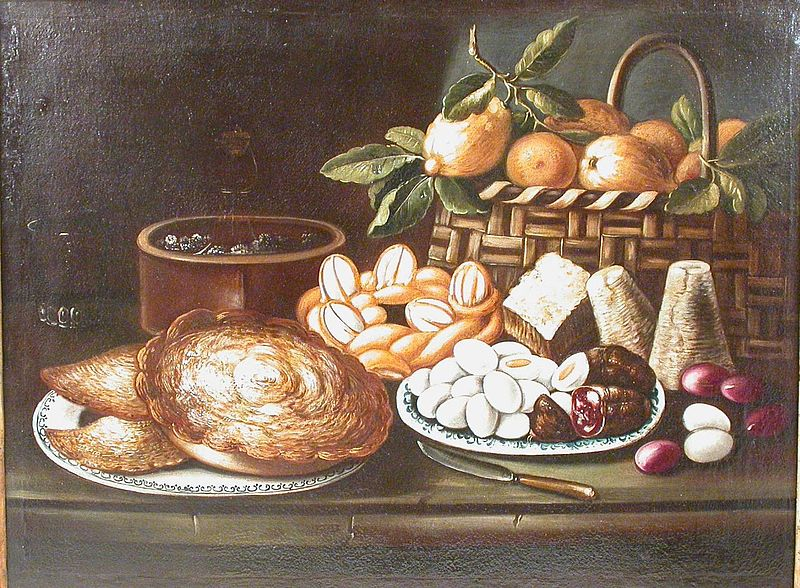
\includegraphics[]{Dispensa_natura_morta.jpg}
			\captionof{figure}{Tommaso Realfonso - Dispensa con dolci, uova, salame, formaggi, ghiacciaia e canestro di limoni.}
		\end{minipage}
		\hfill
		\begin{minipage} {0.4\linewidth}
			\includegraphics[scale=0.25]{Morte_di_Adone.jpg}
			\captionof{figure}{Francesco Gessi - Morte di Adone.}
		\end{minipage}
		
	\end{minipage}
	
	\item \textbf{Per eventuali laboratori creativi con bambini gli può essere fornito un dettaglio dell'opera per poi far sì che vadano a ricercare essa all'interno del museo.}
	
	
	\end{enumerate}
\newpage
\listoffigures

\end{document}